%% DC 16: In a perfect world, we would go back and relate our results specifically to some of the work we claim raises related questions at the beginning of the Overview section to show what we learned that's either different or similar, and in a perfect world this would lens in on how our analysis differed from theirs in ways that helps us see The New Thing to help make the case for our analysis (although I think we do a reasonable job of that as is just through doing the analysis).  
%%
%% This is probably below "make figures readable and current text clear" in priority; if you do wind up having energy for it, I would probably do it in the discussion when we re-surface the main results we want to comment on, especially if you do the methods comparison part.    

\section{Average posts per user}

\begin{figure*}[!tb]
\centering
\subimage[width=0.48, scale=0.45]{./images/avr_posts_per_user_over_time_total.eps}
\subimage[width=0.48, scale=0.45]{./images/avr_posts_per_user_user_ref_total.eps}
\caption{In Figure (a), monthly average posts per active user over clock time. In Figure (b), the monthly average posts per active users in the user-time referential, i.e., message creation time is measured relative to the user's first post.  Each tick in the x-axis is one year.  In both figures (and all later figures), we consider only active users during each month; users that are either temporarily or permanently away from Reddit are not included.}
\label{fig:overall_posts}
\end{figure*}

In this section, we will use a common metric of user activity in online communities, the number of posts per user over time. Approaches that consider the total number of posts per user in a particular dataset \cite{Gruhl2004} and that analyzes the variation on the number of posts per user over the days \cite{Guo2009} have been applied to online social networks.

As we will see, both visualizing behavior relative to a user's join time rather than calendar time and using cohorts provide additional insight into posting activity in Reddit compared to a straightforward aggregate analysis based on clock time.

\subsection{Calendar versus user-relative time}

We start with a common analysis used in this kind of work: aggregating behavior in the community based on calendar time.  Figure~\ref{fig:overall_posts}a shows the average number of posts per month by active users in that month.  Taken at face value, this suggests that over the first few years of Reddit, users became more active in posting, with per-user activity remaining more or less steady since mid-2011.

This average view hides several important aspects of users' activity dynamics. Previous work has looked into behavior relative to the user creation time. It has been shown that edge creation time in a social network relative to the user creation follows an exponential distribution \cite{Tomkins2008}. User lifetime, however, does not follow a exponential distribution and some types of user content generation follow a stretched exponential distribution \cite{Guo2009}. In Figure~\ref{fig:overall_posts}b, we show a different view that emphasizes the trajectory over a user's lifespan.  Here, we scale the x-axis not by clock time, as in the left figure, but by time since the user's first post: ``1'' on the x-axis refers to one year since the user's account first post, and so on.

One caution about interpreting the graphs that are relative to the user's start time is that the amount of data available rapidly decreases over time as users leave the community, meaning that values toward the right side of an individual data series are more subject to individual variation.  A tempting conclusion at this point is that the longer a user survives, the more posts they make over time.  This conclusion, however, is incorrect; we will present a more nuanced description of what is happening informed by cohort-based analyses.

\subsection{New cohorts do not catch up}

\begin{figure*}[!tb]
\centering
\subimage[width=0.48, scale=0.45]{./images/avr_posts_per_user_over_time_cohorts.eps}
\subimage[width=0.48, scale=0.45]{./images/avr_posts_per_user_cohorts.eps}
\caption{Figure (a) shows the average number of posts per active users over clock time and Figure (b) the active users in the user-time referential, both segmented by users' cohorts. The user cohort is defined by the year of the user's creation time.  For comparison, the black lines represent the overall averages from Figure~\ref{fig:overall_posts}.}
\label{fig:avr_posts_per_user_over_time_cohorts}
\end{figure*}

Figure~\ref{fig:overall_posts}b suggests that older users are more active than newer ones, raising the question of whether newer users
will eventually follow in older users' footsteps.  Analyzing users' behavior by cohort is a reasonable way to address this question.  

Figure~\ref{fig:avr_posts_per_user_over_time_cohorts}a shows our first attempt at this analysis.  This Figure already shows a significant cohort effect: users from later cohorts appear to level off at a significantly lower posting average than users from earlier cohorts.  It suggests that newer users probably will not ever be as active on average as older ones.

However, Figure~\ref{fig:avr_posts_per_user_over_time_cohorts}a also has an awkward anomaly, the rapid rise in the average number of posts during each cohort's first calendar year, especially in December.  
Combing cohort segmentation with user-referential analysis, as in Figure~\ref{fig:avr_posts_per_user_over_time_cohorts}b, helps smooth out this anomaly and aligns cohorts with each other.  Doing this alignment makes clear that differences between earlier and later cohorts are apparent early on.

\subsection{Does tenure predict activity, or vice versa?}

%% DC 15: Calling this out was really nice; very subtle.
These graphs still support the tempting conclusion that users become more active the longer they exist in Reddit, and they do not explain the very rapid increase in posting activity in the first few months.  An alternative hypothesis, inspired by the ``Wikipedians are Born, not Made'' paper \cite{Panciera2009}, is that individual users come in with different posting propensities, and the rise over time is not that individual users become more active but that low-activity users leave the system.  To examine this, we further segment each cohort by the number of years they were active in the system, as defined by the difference between their first and last post times.
 
Figure~\ref{fig:avr_posts_per_user_for_surviving_year} shows this analysis for the 2010, 2011 and 2012 cohorts\footnote{We only show these figures for the sake of saving space, but the same trends are observed in the other cohorts.}.  Across all cohorts and yearly survival sub-cohorts, users who leave earlier come in with a lower initial posting rate.  Thus, the rise in average posts per active user is driven by the fact that users who have high posting averages throughout their lifespan are the ones who are more likely to survive.  As the less active users leave the system, the average per active user increases.  In other words, the correct interpretation of Figure~\ref{fig:overall_posts}b isn't that longer-lived users post more.  It actually is that users who post more---right from the beginning---live longer. 

\begin{figure*}[!tb]
\centering
%\subimage[width=0.31, scale=0.29]{./images/avr_posts_per_user_for_surviving_year_for_2008.eps}{2008 cohort}
%\subimage[width=0.31, scale=0.29]{./images/avr_posts_per_user_for_surviving_year_for_2009.eps}{2009 cohort}
\subimage[width=0.31, scale=0.29]{./images/avr_posts_per_user_for_surviving_year_for_2010.eps}{2010 cohort}
\subimage[width=0.31, scale=0.29]{./images/avr_posts_per_user_for_surviving_year_for_2011.eps}{2011 cohort}
\subimage[width=0.31, scale=0.29]{./images/avr_posts_per_user_for_surviving_year_for_2012.eps}{2012 cohort}
\caption{Each Figure corresponds to one cohort, from 2010 to 2012, left to right. The users for each cohort are further divided in groups based on how long they survived: users that survived up to 1 year are labeled 0, from 1 to 2 years are labeled 1, and so on.  For all cohorts, longer-tenured users started at higher activity levels than shorter-tenured ones.}
\label{fig:avr_posts_per_user_for_surviving_year}
\end{figure*}

%% DC 15: Trying to make this argument clearer.  I'm not positive I believe it but it's interesting. 
Combining Figure \ref{fig:avr_posts_per_user_for_surviving_year}'s insight that the main reason why these curves increase is because the low posting users are dying sooner with the earlier observation that the stable activity level is lower for newer cohorts suggests that low-activity users from later cohorts tend to survive longer than those from earlier cohorts.  That is, people joining later in the community's life are less likely to be either committed users or leave than those from earlier on: they are more likely to be ``casual'' users that stick around.

\section{Comment length}

\begin{figure*}[!tb]
\centering
\subimage[width=0.48, scale=0.45]{./images/avr_comment_size_over_time_cohorts.eps}
\subimage[width=0.48, scale=0.45]{./images/avr_comment_size_cohorts.eps}
\subimage[width=0.31, scale=0.29]{./images/avr_comment_length_for_surviving_year_for_2010.eps}{2010 cohort}
\subimage[width=0.31, scale=0.29]{./images/avr_comment_length_for_surviving_year_for_2011.eps}{2011 cohort}
\subimage[width=0.31, scale=0.29]{./images/avr_comment_length_for_surviving_year_for_2012.eps}{2012 cohort}
\caption{Figure (a) shows the average comment length over clock time and Figure (b) from the user-referential time. Both figures show the cohorted trends and the overall users trends.  The overall average length per comment decreases over time, although for any individual cohort, it increases after a sharp initial drop. Figure (c), similar to Figure \ref{fig:avr_posts_per_user_for_surviving_year}, shows the monthly average comment length for active users in the cohorts of 2010, 2011 and 2012, segmented by the number of years that the user survived in the network.  Opposite the analysis for average posts, which showed that low-activity users were the first to leave Reddit, here, people who start out as longer commenters are \textit{more} likely to leave.}
\label{fig:comment_length}
\end{figure*}
%% DC 15: You do want the _key_ point to come out in the caption. 

Activity as measured by the average number of posts per user is one proxy for user effort.  Comment length can also be considered as a proxy for user effort in the network.  Users that type more put more of their time in the network, contribute with more content, and might create stronger ties with the community.  Thus, we investigate how comment length has changed in the community over time, both overall and by cohort. 

\subsection{Comment length drops over time}

%% DC 15: The per-cohort by calendar time analysis isn't as interesting to me, just the overall one, because that's what's going to really make the Simpson's paradox for us.  (Especially if we drop our speculation that people coming in start commenting at average lengths they see at their moment of inception.  I'm going to put that back for now, at the end where you talk about understanding why. ).
Figure \ref{fig:comment_length}a shows the overall comment length in Reddit over time (the black line) and the overall length per cohort. 
Based on the downwards tendency of the overall comment length in Figure \ref{fig:comment_length}a, one might infer that users' commitment to the network is decreasing over time, or that there is some community-wide norm toward shorter commenting. 

This, however, might not be the best way to interpret this information. Figure \ref{fig:comment_length}b shows the comment length per cohort based on the user referential time. An important thing to notice here is that younger users start from a lower baseline comment length than older users. Together with the fact that recent Reddit has experienced exponential growth, the weight when evaluating the overall average for Figures \ref{fig:comment_length}a and \ref{fig:comment_length}b as the years go by is shifted towards the length of the ever-growing younger generation; this younger generation brings the average down since they writing less on average.

\subsection{Simpson's Paradox: the length also rises}

Let us go back to Figure~\ref{fig:comment_length}a, which shows the overall average comment length on Reddit over time. We see a clear trend towards declining length of comments in the overall line (the black line that averages across all users).
%% DC 15: This is a little harder to say "across all users" because of the individual cohort views in Fig a here.  I still think removing them there makes the story quite a bit clearer, and the per-cohort info is visible in Fig b.
This could be a warning sign for Reddit community managers, assuming longer comments are associated with more involved users and healthier discussions. A data analyst looking at these numbers might think about ways to promote longer comments on Reddit. 

However, in Figure~\ref{fig:comment_length}b, we saw that average comment length increases over time for every cohort. While later cohorts start at smaller comment length, after an initial drop, all cohorts show positive trends towards writing longer comments over time.  This is puzzling: when each of the cohorts exhibits a steady increase in their average comment length, how can the overall mean comment length decrease?  This anomaly is an instance of the Simpson's paradox \cite{simpson1951}, and occurs because we fail to properly condition on different cohorts when computing mean comment length. 

\begin{table}[!tb]
\centering
\tabcolsep=0.07cm
\singlespacing
\fontsize{9pt}{11.5pt}\selectfont
\begin{tabular}{|c|c|c|c|c|c|c|c|c|c|}
\cline{2-9}
\multicolumn{1}{c|}{} & \multicolumn{8}{c|}{Cohorts} \\ \hline
Year & 2007 & 2008 & 2009 & 2010 & 2011 & 2012 & 2013 & 2014 & Overall\\ \hline
2007 & 220 & - & - & - & - & - & - & - & 220 \\ \hline
2008 & 208 & 198 & - & - & - & - & - & - & 204 \\ \hline
2009 & 224 & 204 & 201 & - & - & - & - & - & 208 \\ \hline
2010 & 223 & 204 & 189 & 184 & - & - & - & - & 193 \\ \hline
2011 & 233 & 211 & 199 & 184 & 167 & - & - & - & 182 \\ \hline
2012 & 241 & 221 & 212 & 197 & 173 & 167 & - & - & 178 \\ \hline
2013 & 244 & 225 & 214 & 199 & 177 & 167 & 164 & - & 174 \\ \hline
2014 & 246 & 229 & 217 & 204 & 183 & 172 & 165 & 176 & 176 \\ \hline
\end{tabular}
\caption{Evolution of the average throughout the years for each cohort. Each column here is one cohort and each line is one year in time. Cohorts only start having data on the cohort year, therefore the upper diagonal is blank. On the right column we see the overall average for all users.}
\label{tab:simpson}
\end{table}

Table~\ref{tab:simpson} provides some clues to what might be going on. When we move down the rows, we observe an increasing tendency in each cohort column. It means that the average comment length increases for these users. However, when we move right through the columns, people in later cohorts tend to write less per comment. If we were to average each row, we would still get an overall increasing comment length per year, but that is not what we see in the overall column. What happens here is that the latter cohorts have many more users than earlier ones. Since their numbers increase year by year, we have a much larger contribution from them towards comments, compared to users of earlier cohorts. This uneven contribution leads to the paradox we observed in Figure~\ref{fig:comment_length}a. 

Without the decision to condition on cohorts, one would have gathered an entirely wrong conclusion. People are not writing less as they survive, rather those who tend to write less are joining the community in much larger numbers. Knowing this, one may focus on better onboarding processes for newcomers, or try to learn why users in later cohorts tend to write smaller comments on average.  

%% DC 15: Caption and figure don't line up, making it hard for me to know what to focus on here.
\begin{figure*}[!tb]
\centering
\subimage[width=0.48, scale=0.45]{./images/comments_per_submissions_over_time_cohorts.eps}
\subimage[width=0.48, scale=0.45]{./images/comments_per_submissions_cohorts.eps}
\subimage[width=0.23, scale=0.23]{./images/comments_per_submissions_for_surviving_year_for_2008.eps}{2008 cohort}
\subimage[width=0.23, scale=0.23]{./images/comments_per_submissions_for_surviving_year_for_2009.eps}{2009 cohort}
\subimage[width=0.23, scale=0.23]{./images/comments_per_submissions_for_surviving_year_for_2010.eps}{2010 cohort}
\subimage[width=0.23, scale=0.23]{./images/comments_per_submissions_for_surviving_year_for_2011.eps}{2011 cohort}
\caption{Figure (a) shows the average comment per submission ratio over clock time and Figure (b) from the user-referential time. Both figures show the cohorted trends and the overall users trends. Figure (c), similarly to Figure \ref{fig:avr_posts_per_user_for_surviving_year}, shows the 2008, 2009, 2010, and 2011 cohorts, segmented by the number of years a user in the cohort survived.  As with average posts per month, users who stay active longer appear to start their careers with a relatively high comment-to-submission ratio than users who abandon Reddit sooner.  Unlike that analysis, however, the early 2008 cohort ends up below the later cohorts.}
\label{fig:comments_submissions}
\end{figure*}

\subsection{New users burn brighter}
As with the posting per user, we can not say if the increase in the curves seen in \ref{fig:comment_length}b are due to the lower effort users dying first or because users are writing more as they live on the network. To answer this, \ref{fig:comment_length}c allow us to make two important observations: first, \textit{comment length does increase inside of each cohort}, no matter how long the user survives. Secondly, as a general trend, \textit{users that make longer comments inside of each cohort die faster}. This is quite surprising, given that we would expect people to put less effort when they are more likely to stop using the network.

\section{Kinds of contributions}

One common question from the literature is what sorts of activities users engage in, for instance, to categorize users into roles they play in the community\cite{Welser2011}.

\subsection{Over time, responsiveness increases}
Consider the case of Usenet: people who never start threads and only respond play the role of answerer, while there are other roles that include fostering discussion \cite{Welser2007}. These might naturally map onto people who primarily comment and who primarily submit in Reddit, respectively.  While submissions can be considered new content that an author generates, a comment can be considered as a contribution to an existing content from another author.

Since the total number of comments always surpasses the number of submissions, Figure \ref{fig:comments_submissions}a shows the evolution of the overall and cohorted ratio of the average number of comments a user makes for each submission they make over time from 2008 until 2013. Here we see that users who most prefer commenting to submitting come from 2009, 2010 and 2011, and we observe that, over time, the average ratio of comments to submissions increases both overall and per-cohort for active users.

Again, we analyze our data from the user-time referential, as seen in Figure \ref{fig:comments_submissions}b. It shows a clear pattern for users in earlier cohorts to have a lower comment per submission ratio than users in later cohorts ones, given that they both survived the same amount of time.  Surviving users from later cohorts also exhibit a more rapid increase in comments per submission than those from earlier cohorts.  In particular, the 2008 and 2009 cohorts increase much more slowly over time than those from 2010 onwards; later cohorts are more similar (although the 2012 and 2013 cohorts may level off lower than 2011 based on the limited data we have). 
%% DC 15: Don't understand what you mean here.
% Also, cohorts from 2010 onwards show a much more similar evolution when compared with 08 and 09. Our observation that 2009, 10 and 11 are the main comenters therefore is mainly due to the fact that users in those cohorts are the ones that survived longer.  

\subsection{Comment early, comment often}

Figure \ref{fig:comments_submissions}c shows the cohorts from 2008, 2009, 2010 and 2011 segmented by surviving year.  Three interesting observations arise from these data.  First, we see that just as in the analysis of average posts per user, the users who survive the longest in each cohort are also the ones who hit the ground running.  They start out with a high comment-to-submission ratio relative to users in their who abandon Reddit more quickly.  This suggests that both the count of posts and the propensity to comment might be a strong predictor of user survival.

Second, and unlike the case for average post length, surviving users' behavior changes over time.  Figure~\ref{fig:avr_posts_per_user_for_surviving_year} shows that even for the most active users, they come in at a certain activity level and stay there, perhaps even slowly declining over time.  Here, the ratio of comments to submissions increases over time; combined with the observation that overall activity stays steady, this suggests that the ratio is changing because people \textit{substitute} making their own submissions for commenting on others' posts.

Finally, this increase is most pronounced for the earliest cohorts from 2008 and 2009, with ratios more than doubling over their first year, much more than the change for later cohorts.  Still, the ratio for these earlier cohorts never rises to the level it does for surviving users from later cohorts.  

%% DC 15: Here's an interesting history from someone.  https://www.reddit.com/r/TheoryOfReddit/comments/1a7aoj/retracing_the_evolution_of_reddit_through_post/
 
%% DC 15: I don't think we shoult try to analyze this here; we should just point out that it removes the anomaly.  It's hard to really talk through this without having done the cohort-in-cohort analysis, so I'll move that as a question there.
%Based on Figure~\ref{fig:overall_posts}b, we might guess that this is because users who are active only a short time 
%are lower-activity on average than later ones, and low-activity users are joining every month during the first year of the cohort, dragging the average down.  
%To support that it is indeed the case that these users are causing these effects, we need yet other representations of the users' evolution.
%% DC 15: Tried to reword to make clearer. 

%% DC 15: I don't actually believe that this is what explains what's happening in Figure (a).
%These account for the lower values in the initial cohort year in Figure~\ref{fig:avr_posts_per_user_over_time_cohorts}a. 

%% DC 15: This isn't quite right; folks grow, especially in 2011 -- but at a slower rate than the first two cohorts.
%2010 and 11 are consistent with the following years, with users that survive longer rapidly leveling at higher values while users that survive less also rapidly leveling at lower values. For 2008 and 09, however, this is not the case. Users actually increased their commenting behavior in the early years. Still, users that survived longer show a higher commenting behavior than the ones that survived a shorter period.

%% DC 15: Not sure I believe this one; most of that is driven by the last year of data for each sub-cohort, which has the right-censoring problem. 
% It is also important to notice that Figure \ref{fig:avr_posts_per_user_for_surviving_year} shows that users are more likely to post less as they live on.

%% DC 10: There is a mysterious question about why 2008 ramps up more slowly, that I would interpret in the "there was less to comment on" framing that we've chatted about before.  You could actually do an analysis to test this, where for each user, the number of posts in a month is normalized by the number of posts made in Reddit in that month: that is, how active is the user relative to the total amount of activity in Reddit.  This is _not_ a linear scaling when the analysis is relative to the user's initial start date, and I would be curious to see what it showed.
%% Sam 14: There is an important point here that I think we did not explore properly. The fact that we count surviving users makes the interpretation of the user-time referential figures hard. This happens because we do not know if it is increasing because surviving users are indeed increasing their activity or because the ones dying are the low activity ones. That is why I made the sets of figures for each cohort. But there is more: the cohorted curves from the user-referential (particularly 2008) might not be increasing because in these cohorts the low activity keep around, pulling the average down, but they don't die, while in some other cohorts they might die and let the average go up. This kind of comprimises some of these analysis in my opinion.
%% Actually, when we control for the surviving time in the set of pictures for each cohort, we see that the posting per user is going down. This actually means that, for the average to increase, low activity users have to die, and if it doesn't increase, it is because low activity users are sticking around.
%% This makes the interpretation of the user-referential cohorted picture more like the ``speed'' at which low activity users are dying entangled with the ``mixture'' of low and high activity users that joined the network. If the curve goes up fast, it means that the low activity die faster in that cohort. If it goes up slower, they die more slowly. How fast and how slow they can go also depends on how many low activity versus high activity we have in each cohort. E.g.: 2009 might have 10 low and 10 high, and the 10 low die in the 1st year, so the average jumps to a high value fast, while 2013 might have 1000 low and 10 high, and the low activity are not dying so fast. So it would be natural, even if users were not to die, for 2013 to be lower. If they die, and do so more slowly (assuming independence, which might not be the case), the curve would increase slower than 2009.
%% The curve does say what a user looks like, on average, given that he has survived x time. But does not mean that users are evolving in that way.
%% DC 15: Yep, this all makes sense and I think mostly comes out in the text now.


% This suggests that the increasing tendency in Figure \ref{fig:comments_submissions}b for the cohorts of 2010 and later is mainly due to the death of low-ratio users, but the earlier cohorts also increased due to an actual increase in the commenting behavior of the users, and not only low commenting users dropouts. 

%% Sam 10: It just occurred to me that although the comment size is decreasing, users might be putting just the same amount of effort, just writing more comments. This figure that shows that the newer cohorts comment more might mean that users are actually typing the same amount, but they are pulverizing more their efforts. Might be worth to comment about it, although it obviously raises the question of why we didn't do it. I can try to generate this results on monday, it is likely easy to do so.
%% Sam 10: Thinking again about it, I raise the question of weather users are getting ``lazier'' many times in the text. This should be included. Can probably make up for the removal of the subreddits section due to the fact that we have a lot of default 2008 subreddits.
%% DC 12: The "lazier" question probably is more of a discussion point, but it's one of many processes (and really, _saying_ that people get lazier doesn't explain _why_).
%\begin{figure}[!tb]
%\centering
%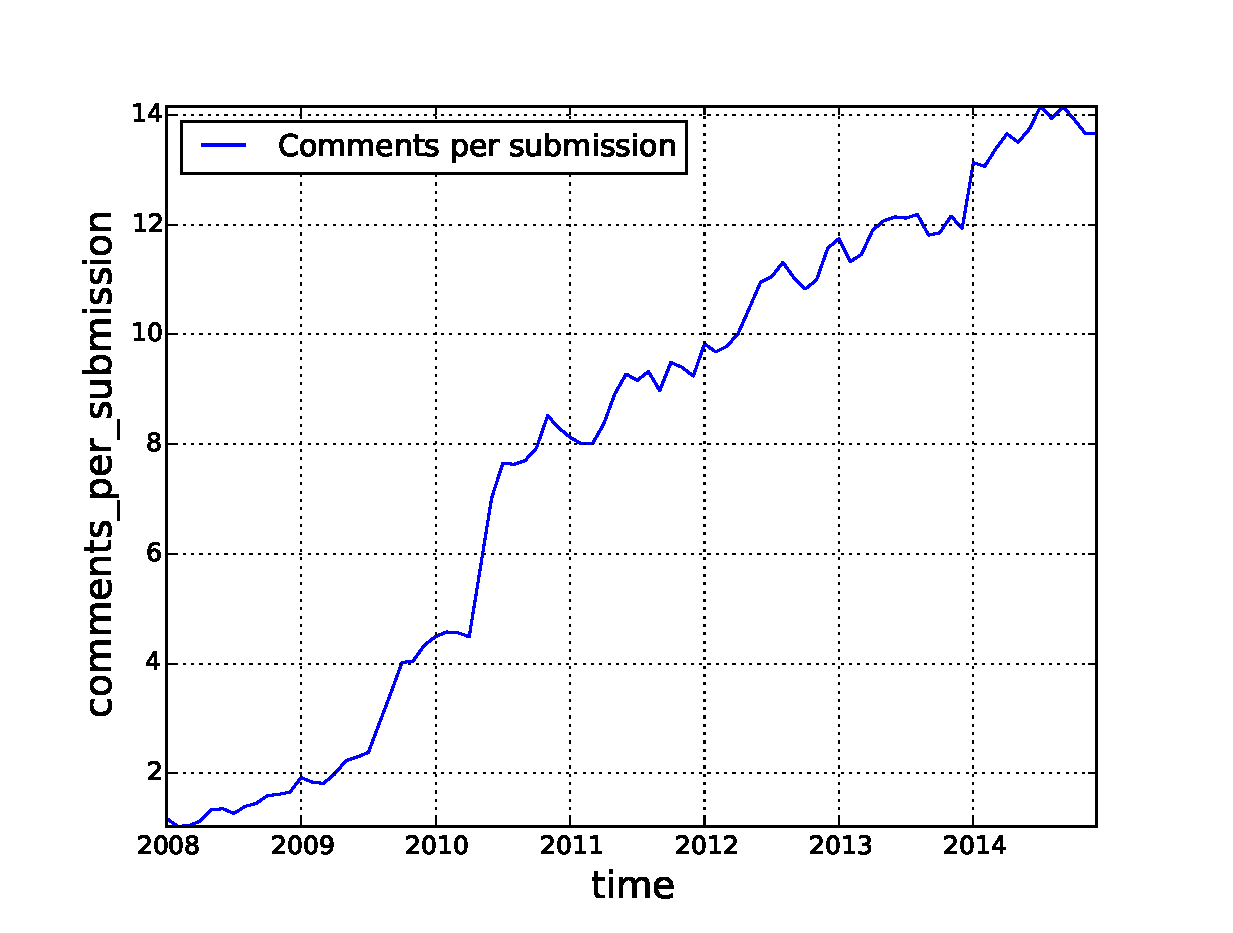
\includegraphics[scale=0.4]{./images/comments_per_submissions_over_time_total.eps}
%\caption{Comments per submission ratio for Reddit over time. We observe an overall increasing trend of comments for each submission. Notice that these should not be interpreted as how many comments each submission gets, but as how many comments users author for each submission --- submissions might get comments a long time after they are posted, by users from different years. This distinction becomes more important when we change the time referential and separate users by cohorts.}
%\label{fig:comments_per_submissions_over_time_total}
%\end{figure}

%% DC 12: Redundant if there's an overall line in the cohort graph.
%\begin{figure}[!tb]
%\centering
%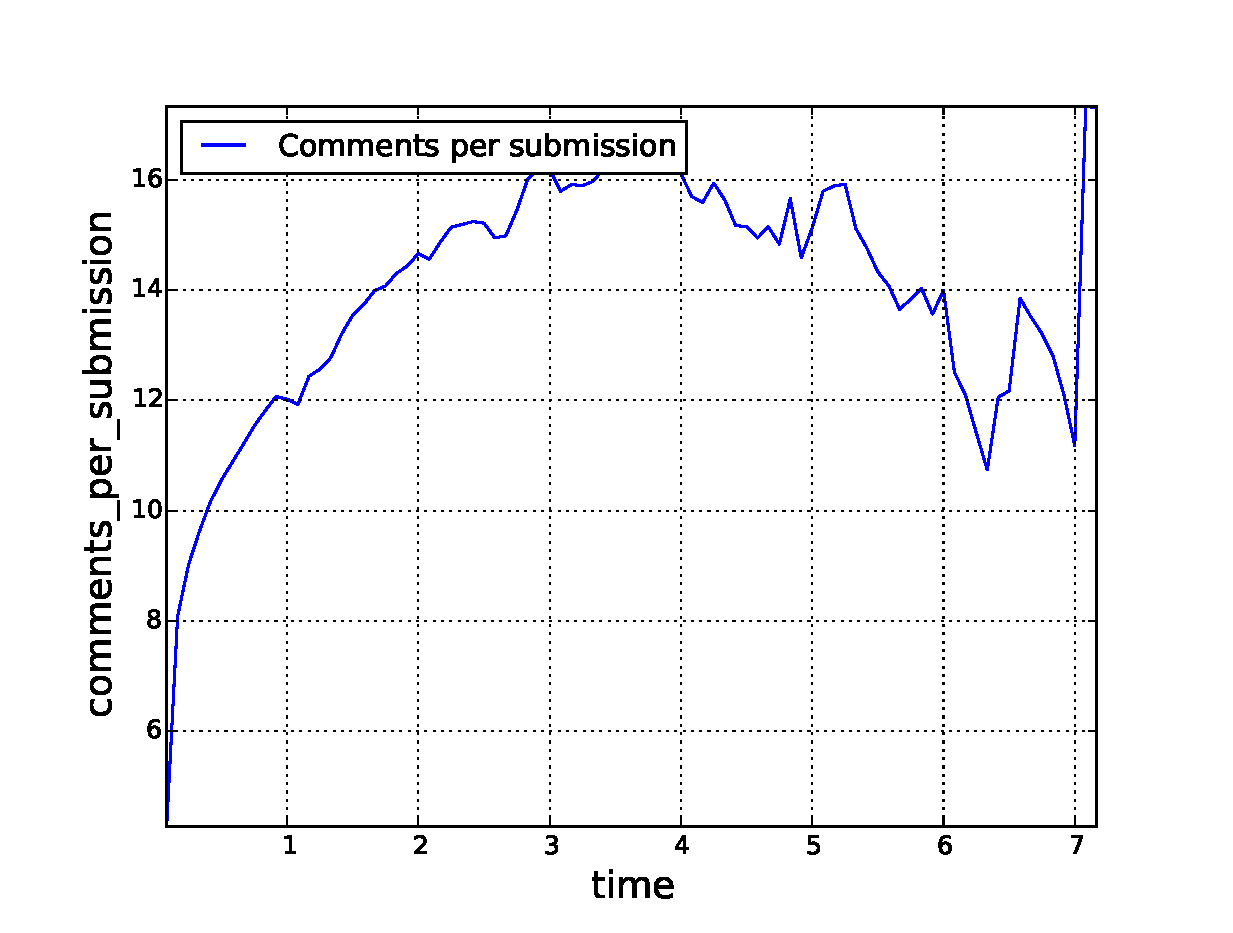
\includegraphics[scale=0.4]{./images/comments_per_submissions_user_ref_total.eps}
%\caption{Comments per submissions ratio from the user referential. This should be interpreted as how many comments a user makes for each submission in their x-th year of existence. We observe an interesting overall trend that peaks between 3 and 4 years of existence. This, however, does not mean that users will necessarily decrease their behavior as they live longer, but that given that a user has survived for x years, what is his/her comment per submission ratio likely to be.}
%\label{fig:comments_per_submissions_user_ref_total}
%\end{figure}

%We have found that segmenting users and subreddits by cohorts on the years that of the first comment highlights significant differences of behavior and help us to understand how Reddit changed over these years.


%Table 1: Number of distinct users that authored comments and submissions segmented by the year of the first post of the user. The Total numbers are based on posting data from 2007 until 2014, corresponding to our full dataset. The Oct 1st, 2014 onwards numbers are based on the last 3 months of data we have, and we consider this as the current, active Reddit.
%
%
%Table 2: Number of distinct subreddits segmented by the year of the first post of the user. The Total numbers are based on posting data from 2007 until 2014, corresponding to our full dataset. The Oct 1st, 2014 onwards numbers are based on the last 3 months of data we have, and we consider this as the current, active Reddit.

%Table indicates that Reddit grew significantly from 2007 until 2012, practically doubling the number of new users per year for each of these years, with similarly significant growth in subreddits. Although the most expansive growth happened in the first years, more than half of the registered users are from the last 2 years, and their behavior is significantly different than previous users, impacting in the overall behavior of the community. For instance, users from the 2014 cohort have a higher tendency to make submissions instead of comments, in contrast with all the previous cohorts.

%\begin{figure}[!tb]
%\centering
%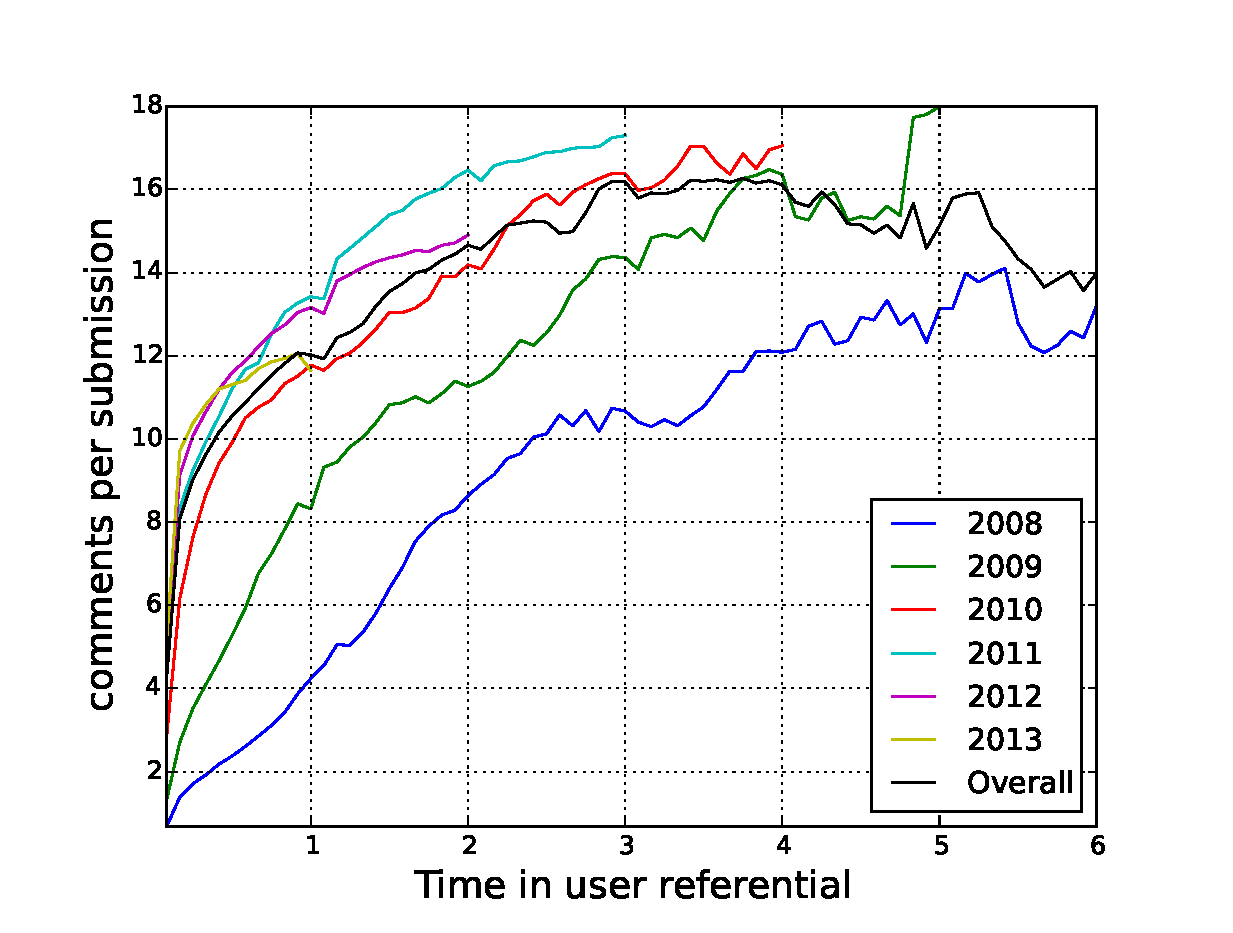
\includegraphics[scale=0.4]{./images/comments_per_submissions_cohorts.eps}
%\caption{Comments per submissions cohorted by user creation year. Here we observe that, unlike the total aggregated graphic, all users are are increasing the number of comments per submissions, but latter cohorts show a much higher level of comments per submissions than earlier cohorts. This brings the initial part of the aggregated user-referential curve up, while the end of the curve consists only of users from the latter cohorts that preset an lower ratio. It is also important to notice that, as these curves move to the right, less comments and submissions exist in the bins, for there are less users that survived for such long periods. This results in some spiky behavior in the rightmost end of some curves due to the reduced amount of data. Just as with the previous user-referential cohort curves, we can not distinguish solely based on this graphic if users are increasing their commenting behavior or if the users that do not comment die earlier. Figure \ref{fig:comments_per_submissions_for_surviving_year} help us to answer this question.}
%\label{fig:comments_per_submissions_cohorts}
%\end{figure}


% DC 12: I'd probably get rid of the survival part for space and coherence.  We're doing analysis that focuses on the surviving users and should just be clear on that and own it.  We can talk about the limitations of that, and questions around how to measure survival, in a discussion maybe.
%\subsection{Users' Survival}
%
%The simplest definition of an active user in Reddit is to set a threshold date and define that every user that posted after that date is an active user and users that do not show any kind of behavior are ``dead''. This, however, is a limited interpretation of how users decide to stay or leave the network, specially if we want to analyse how this behavior changed over time. Also, since our users might always come back to the network at a later time, they might be ``reborn'', that means we have right censored data.
%
%To account for these, we look at a one year window of time for each user. This way, we avoid the right censored data and the possibility that a user might have come back to the network at a later time. Given this, we segment users by their cohort and define that users active in the last 3 months of this one year window are active users. Based on this data manipulation, we present the Kaplan-Meier (cite) survival curve in Figure N.
%
%\begin{figure}[!tb]
%\centering
%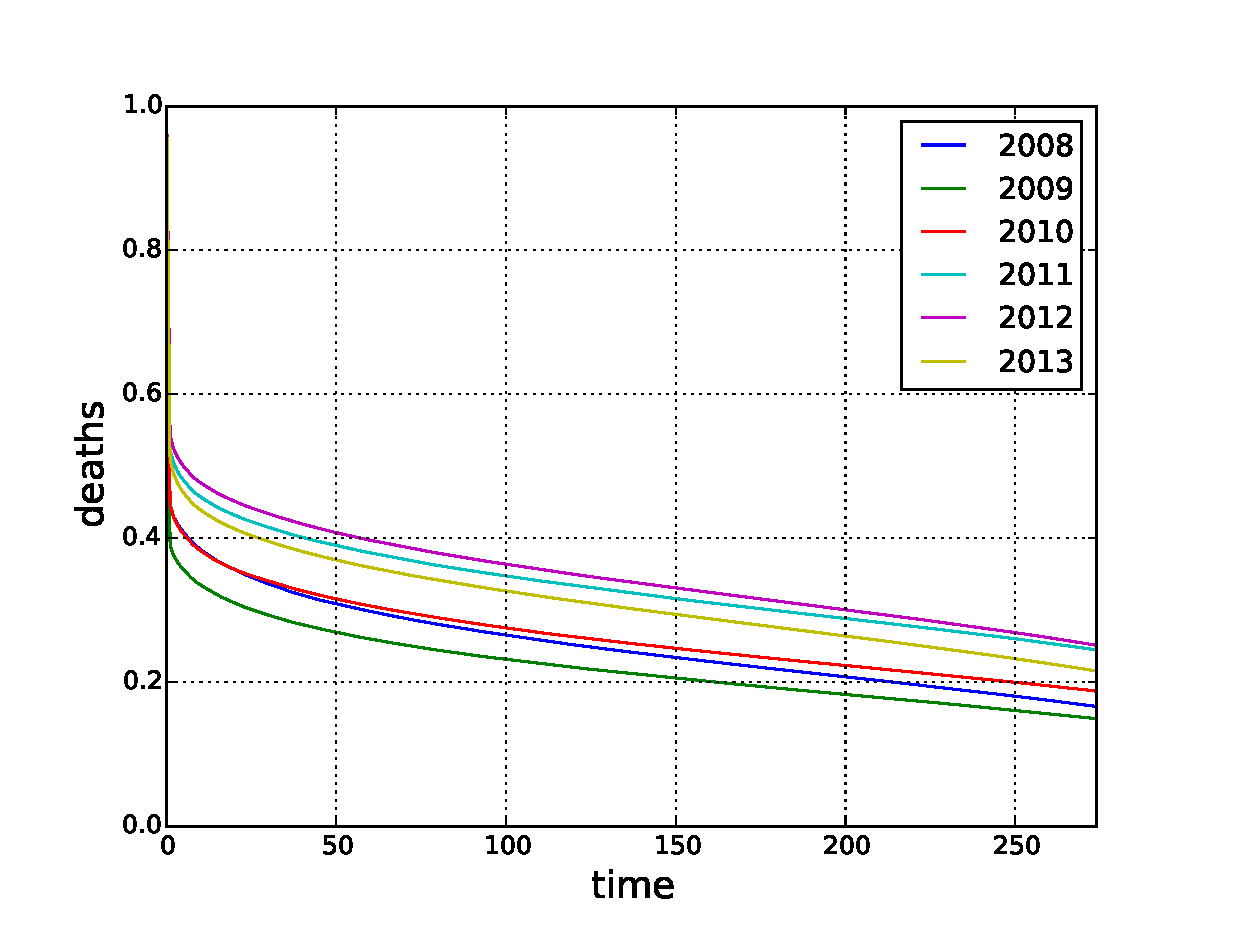
\includegraphics[scale=0.4]{./images/kaplan_meier_users.eps}
%\caption{Kaplan-Meier estimator for one year of posting behavior for each user. Users for which the last posting day was in the first nine months of the one year window are considered ``dead''. This graph shows the percentage of surviving users per number of days since it first posted segmented by the cohort year the user joined the network.}
%\label{fig:kaplan_meier_users}
%\end{figure}
%
%As previously mentioned, Reddit shows a significant number of ``single time users'' that only post once in their existence. This can be seen in the initial drop in the first day. An interesting thing to see is that, although different cohorts level in different survival values, the ``user decay'' is similar throughout all of them. Not only that, but there is a general trend for older cohorts to die faster than younger ones. One possible explanation for that is that early Reddit still lacked in content, with few subreddits to submit and few submissions to comment. This could lead to a higher number of users that did not stayed around after their initial impressions. 
%
% Sam 10: This Figure (c)an go if we don't want/can't give a better explanation regarding survival. It is quite common for survival works to have the hazard plot, although I don't fully understand the values myself.
%\begin{figure}[!tb]
%\centering
%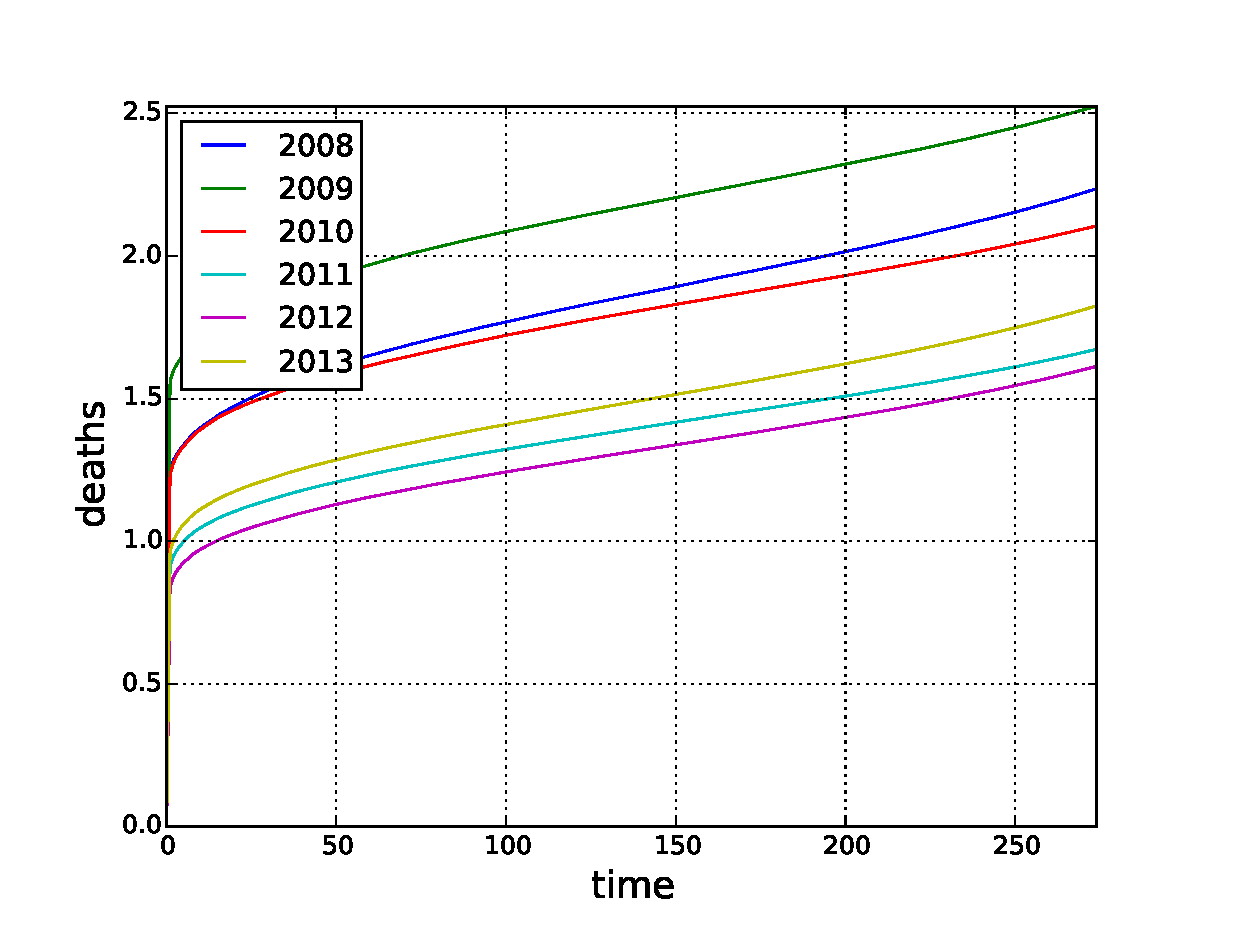
\includegraphics[scale=0.4]{./images/nelson_aalen_users.eps}
%\caption{Nelson-Aalen empirical hazard estimation for the users survival. This curves show the pointwise probability of a user to die in time.}
%\label{fig:nelson_aalen_users}
%\end{figure}
%
% DC 12: Have to stop here.


%%%%%%%%%%%%%%%%%%%%%%%%%%%%%
%%% DC 15: Moving some commented out stuff from above to here for readability in the main line of tex.

%\begin{figure}[!tb]
%\centering
%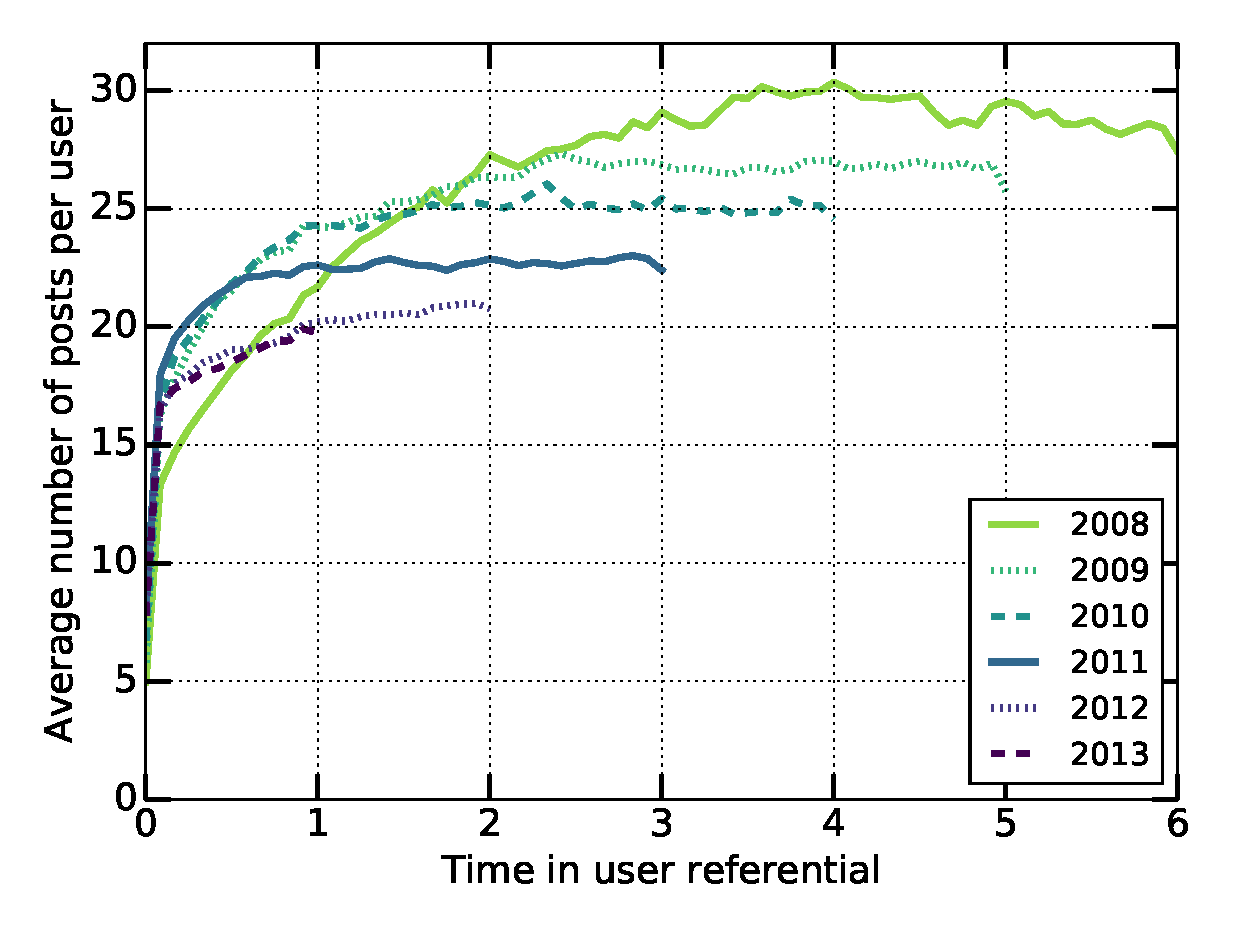
\includegraphics[scale=0.4]{./images/avr_posts_per_user_cohorts.eps}
%\caption{Number of posts per active user for  the overall set of users and cohorts on the user creation date. The x-axis is the time from the user creation referential, i.e., each message creation time is measured in terms of when the user was created. Each tick is one year and we discretized time by month --- the n-th bin holds messages the user wrote in the n-th month. Since we are looking at the user time referential, you can understand this as the surviving users after x time. An interpretation of this says ``users that survived x time are posting on average y messages''. Here we see that, although the 2008 cohort level at a higher value, the evolution of the number of posts took a longer time to increase. The other cohorts seem to follow a more regular pattern after the first year: older users that survived the first year post more on average than younger users that survived the first year. Since we are talking about surviving users, it is not clear from this figure whether these curves increase because the ``low posting users'' are dying earlier or because the users are actually increasing their activity as they live on. To differentiate these cases, Figure \ref{fig:avr_posts_per_user_for_surviving_year} shows, for each cohort, the average posting for users grouped by the number of years they survived in the cohort.}
%\label{fig:avr_posts_per_user_cohorts_relative}
%\end{figure}
%% DC 12: The captions need to be longer than one line, but on average shorter than this.  The first set of figures probably wants longer-than-usual captions to explain what's going on (and you do good to not re-explain things later), but the analysis probably has to go to the body text. 
%\begin{figure}[!tb]
%\centering
%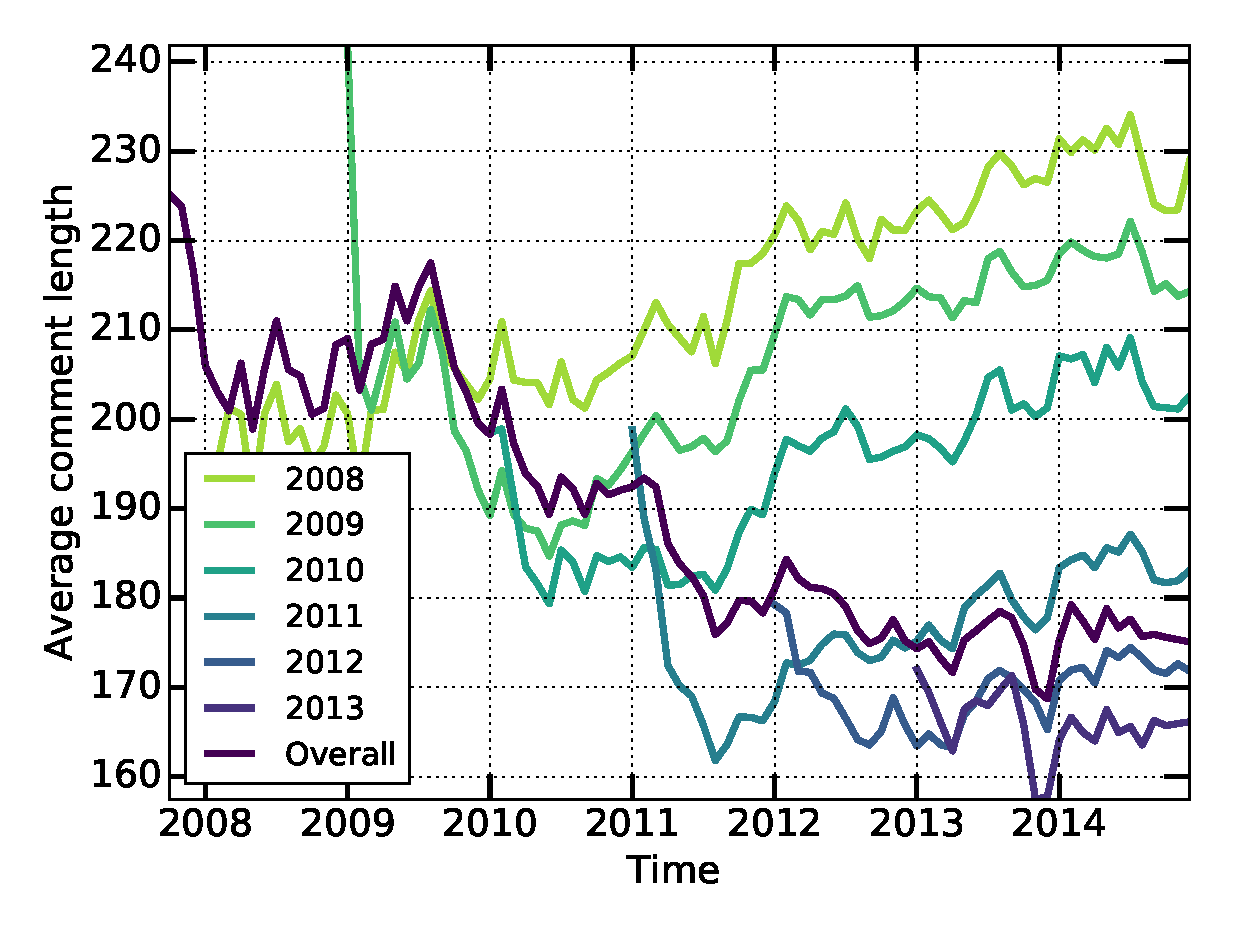
\includegraphics[scale=0.4]{./images/avr_comment_size_over_time_cohorts.eps}
%\caption{Average comment length over time for cohorts on user creation time superimposed over the trend for the total of users. Here we observe how the early existence for each cohort has a reasonable agreement with the overall trend. This might indicate how the new users might be just adopting the community norms regarding comment length.}
%\label{fig:fig_label}
%\end{figure}

%% DC 12: If we're going to focus our attention on the median, then we should re-shoot the graphs to also look at the median.
%% Sam 12: Re-doing everything based on median right now is not really feasible right now. I can redo the table, that is easy.
%\begin{figure}[!tb]
%\centering
%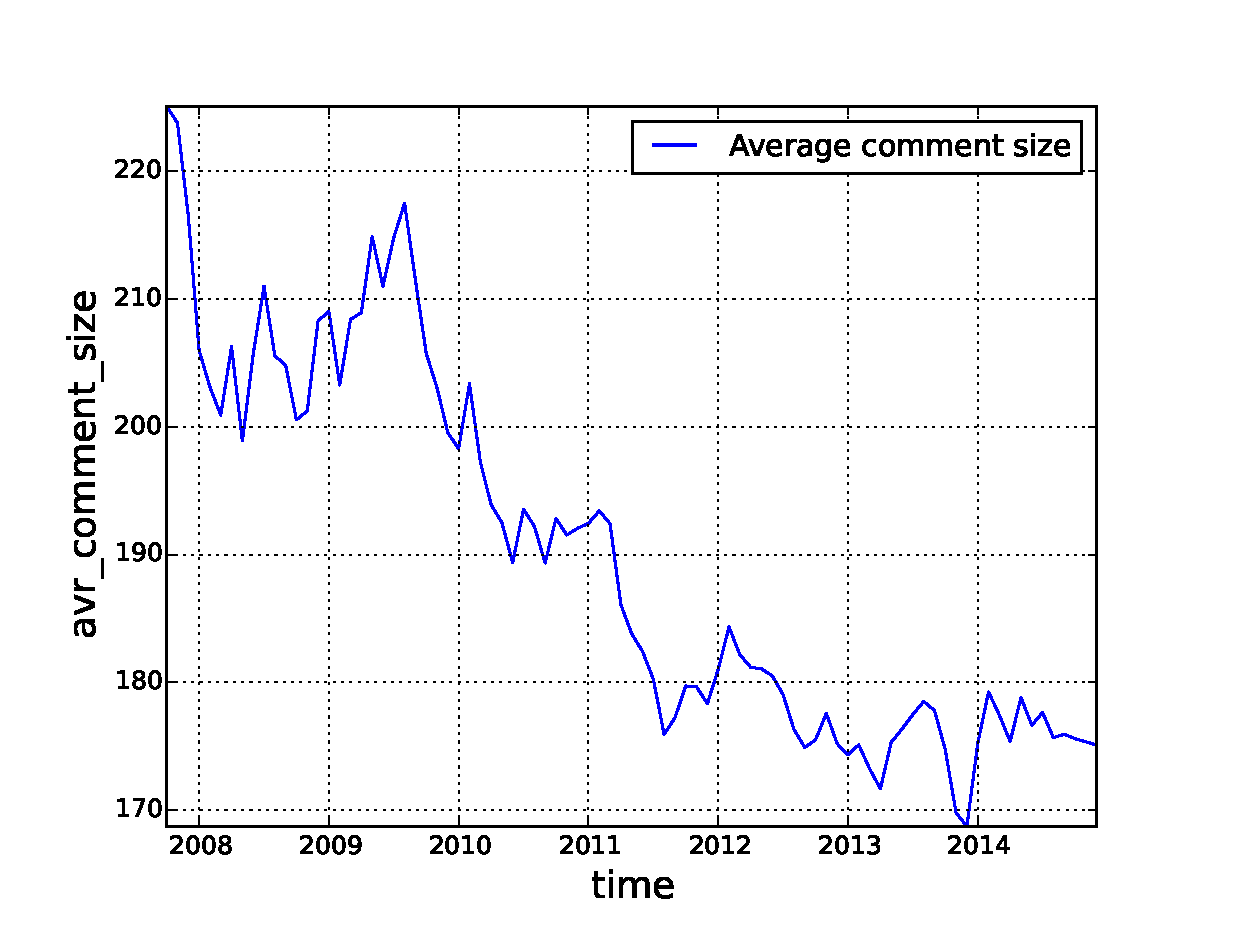
\includegraphics[scale=0.4]{./images/avr_comment_size_over_time_total.eps}
%\caption{Average comment size (number of characters) over time for the Reddit network. We observe that there is a decreasing trend for the average comment size. This means that users, on average, are making smaller comments in Reddit as time passes. This, however, hides important aspects of user behavior over time and does not mean that users, as they survive in the network, write smaller comments.}
%\label{fig:avr_comment_size_over_time_total}
%\end{figure}

%% DC 12: Assuming that we start doing the combined cohort and overall graphs, this figure is no longer needed.
%\begin{figure}[!tb]
%\centering
%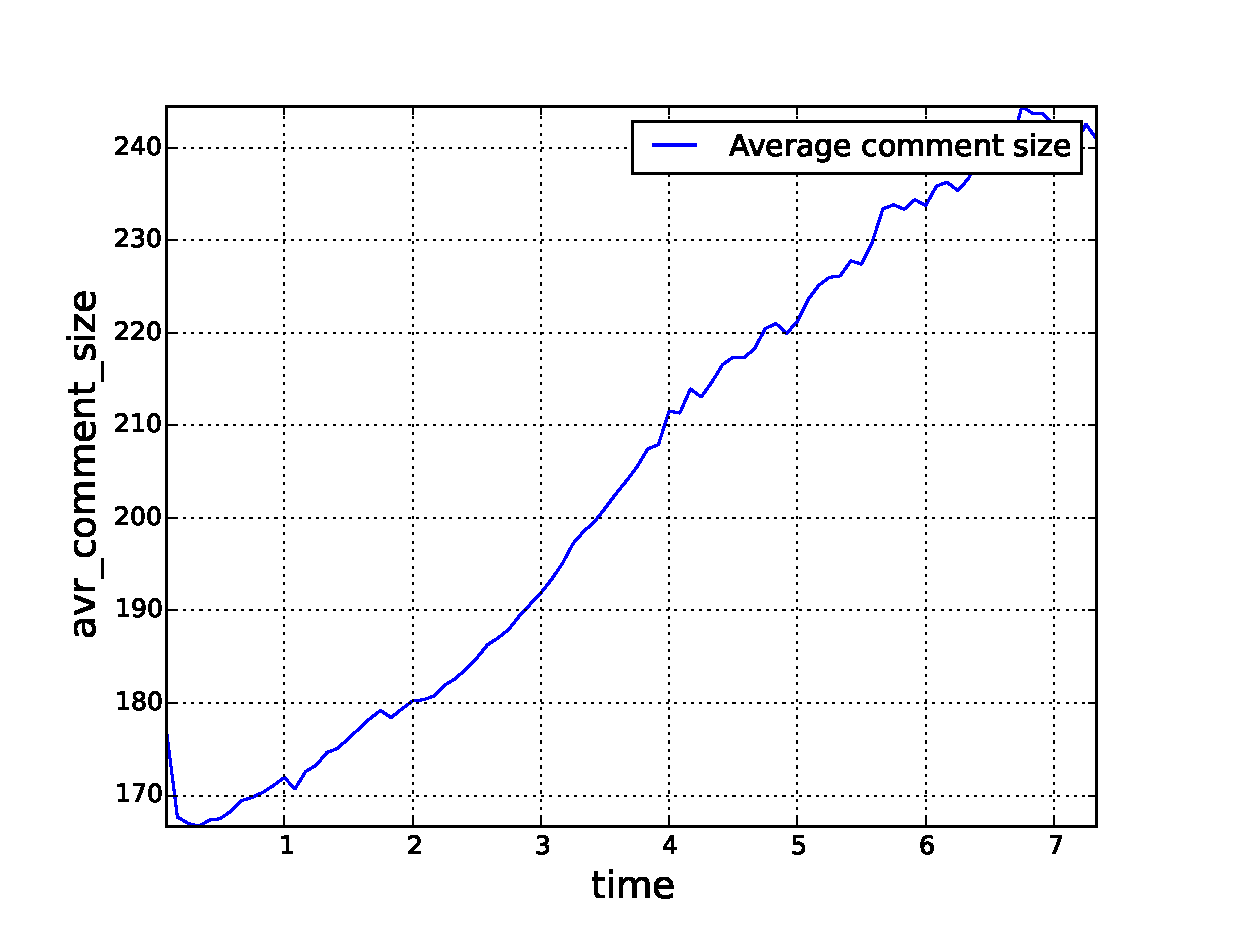
\includegraphics[scale=0.4]{./images/avr_comment_size_user_ref_total.eps}
%\caption{Average comment size from the users time referential. This shows that comment length made by users increase for users that lived longer in the network, save for a small decrease in the initial time. This, however, is also not enough to say that we should expect the average size of the comments in the network to increase since the users that survive write longer comments.}
%\label{fig:avr_comment_size_user_ref_total}
%\end{figure}

%% DC 12: This first one still has no real justification: where is the theory or empirical evidence that demographics is what's going to drive this?
%Some possible explanations for this difference in the starting points could be that older users are, again, sampled from a different demographics that is more committed and willing to spend more effort into developing their virtual identity. 
%% DC 12: Again, this is an interesting speculation, but one that's not at all connected to these data.  When papers try to make these kinds of process speculations that aren't supported by either theory or evidence, they usually are not believable.  In some worlds this one could come in a discussion maybe.
%Also, it could be that it is a natural evolution of the community, as older users have taken most of the main space of interests when it comes to creating new subreddits and starting these communities, new users have it all already made and sometimes might feel intimidated or not motivated to create new topics or communities that already exist or that are less likely to compete with the existing ones. In a way, these new users could behave more as lurkers, while the older users are the ones that laid the foundation of Reddit.

% DC 12: If we're going to focus our attention on the median, then we should re-shoot the graphs to also look at the median.
%\begin{figure}[!tb]
%\centering
%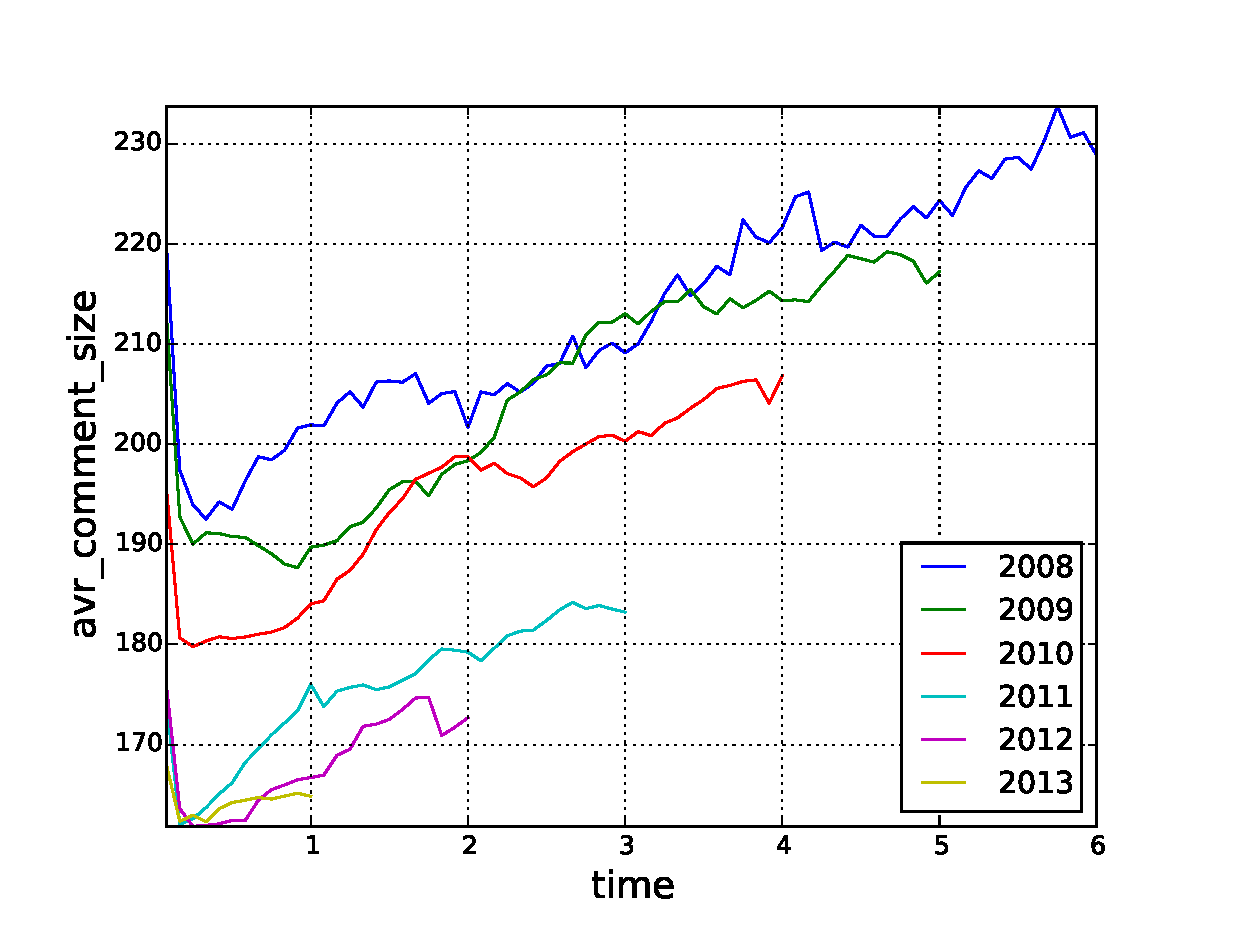
\includegraphics[scale=0.4]{./images/avr_comment_size_cohorts.eps}
%\caption{Average length of comments from the user time referential segmented by user creation cohorts. This figure start to explain why we see different trends in the overall network comment length and user referential overall comment length. It shows that, as users come from latter cohorts, they start from a lower commenting length average compared the the earlier cohorts. This, together with the fact that Reddit is growing exponentially in terms of users means that \textit{we have an influx of users that make smaller comments than the previous generations}, although even for them, as they survive, they make longer comments. Just as for the users' posting average, we can not distinguish based on this graphic alone whether users that make smaller comments leave the network earlier or they indeed write longer comments as they survive. Figure \ref{fig:avr_comment_length_for_surviving_year} sheds some light on this question.}
%\label{fig:fig_label}
%\end{figure}

%% DC 12: 2008 and 2009 awfully noisy here, possibly worth deleting on this one; the 2010-2013 are the money shots here for me.  The first point has already been made by the overall, but the second point is a really interesting observation.
%% The y-axes _have_ to be on the same scale for all of the subfigures, though; this "repeated multiples" style demands that because people are going to expect to be able to visually compare them.
%% They should also be shot at medians if you like median better.

%% DC 12: I am confused by the comment, because I don't know either the percentage like or the wikipedia example parts.
%Sam 9: Still unclear if we should calculate the proportion above and bellow the median of the previous year to have a ``percentage like'' number just as in the wikipedia example. I would like to have this set up as similar as possible as the easiest reference people can find about the subject. A little bit going up by the end, although for some analysis including 2014 and 2007 is a problem, I don't necessarily think it gets in the way here, should we get rid of them?
%\begin{table}[htbp]
%\centering
%\tabcolsep=0.11cm
%\singlespacing
%\fontsize{7pt}{8pt}\selectfont
%\begin{tabular}{|>{\raggedright\centering\arraybackslash}m{1.5cm}|c|}
%\hline
%Year & Median \\ \hline
%2007 & 114 \\ \hline
%2008 & 103 \\ \hline
%2009 & 103 \\ \hline
%2010 & 96 \\ \hline
%2011 & 91 \\ \hline
%2012 & 89 \\ \hline
%2013 & 87 \\ \hline
%2014 & 88 \\ \hline
%\end{tabular}
%\caption{Evolution of the median throughout the years for the whole Reddit dataset.}
%\label{tab:simpson1}
%\end{table}

